\chapter{Casi d'uso}
In questa sezione sono elencati i casi d'uso del progetto MegAlexa dedotti da un'attenta indagine ed analisi da parte dei membri del gruppo sugli attori principali del sistema, sulle loro caratteristiche e possibilità.
Ogni caso d'uso è identificato da un codice univoco e possiede una struttura interna accuratamente definita nel documento Norme Di Progetto 
v1.0.0.

\section{Attori dei casi d'uso}
\textbf{Attori primari}
	\begin{itemize}
	\item \textbf{Utente non autenticato}: si riferisce all'utente del sistema che non ha ancora eseguito il login;
	\item \textbf{Utente autenticato}: si riferisce all'utente del sistema che ha effettuato il login ed è stato autenticato.
	\end{itemize}
\textbf{Attori secondari}
	\begin{itemize}
	\item \textbf{Amazon}:/(da completare)
\end{itemize}


\section{Caso d'uso UC1.1: Scenario principale dell'utente non autenticato}
\begin{figure} [h]
	\centering
	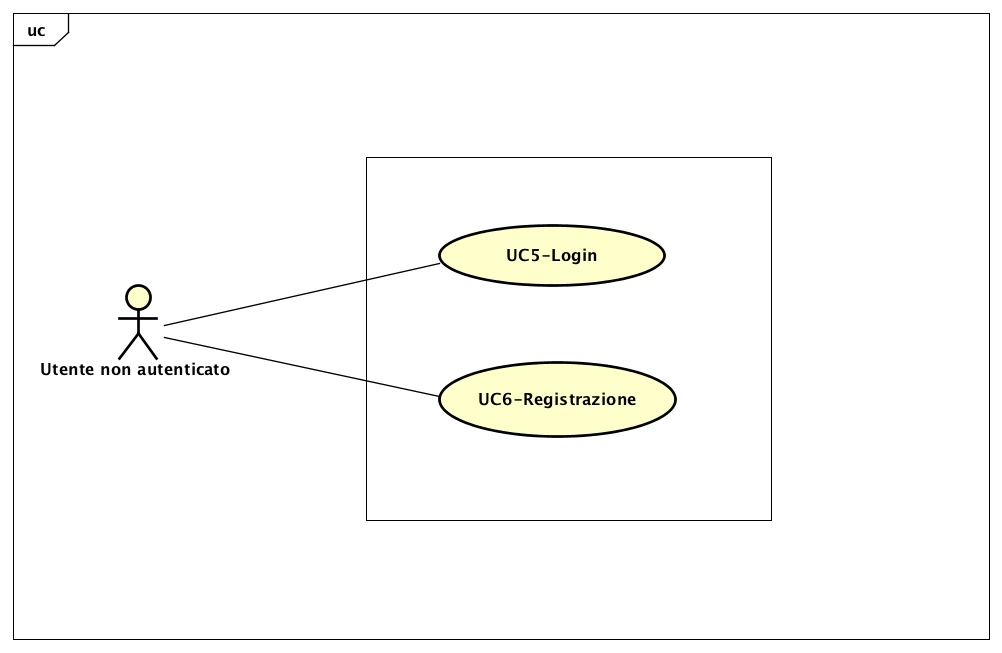
\includegraphics[scale=0.4]{./Diagram/UC1.png}
	\caption{Scenario principale}\label{}
\end{figure}
\begin{itemize}
	\item \textbf{Attori primari}: Utente non autenticato;
	\item \textbf{Attori secondari}: DataBase??;
	\item \textbf{Descrizione:} Un utente non  autenticato può registrarsi al nostro servizio se non ha ancora un account o effettuare il login, nel caso fosse già registrato;
	\item \textbf{Precondizione:} L'applicazione è avviata e pronta all'uso;
	\item \textbf{Flusso principale degli eventi}:
		\begin{enumerate}
			\item L'utente ha la possibilità di: Registrazione (UC1.3);
			\item L'utente ha la possibilità di: Login (UC1.4).
		\end{enumerate}
		\item \textbf{Postcondizione:} L'applicazione ha ricevuto tutte le informazioni dell'utente non autenticato sulle operazioni che vuole eseguire.
\end{itemize}
\section{Caso d'uso UC 1.1}

\section{Caso d'uso UC2: Scenario principale dell'utente autenticato}
\begin{itemize}
	\item \textbf{Attori primari}: Utente autenticato;
	\item \textbf{Attori secondari}: ;
	\item \textbf{Descrizione:} L'attore può creare e modificare un workflow, modificare i propri dati personali ed eseguire il logout.
	\item \textbf{Precondizione:}
	\item \textbf{Flusso principale degli eventi}:
	\begin{enumerate}
		\item L'utente può creare un Workflow(UC1.5);
		\item L'utente può modificare un Workflow(UC1.6);
		\item Modifica dati personali(UC1.7 );
		\item Logout(UC1.8);
	\end{enumerate}
	\item \textbf{Postcondizione:} 
	\item \textbf{Estensioni}:

\end{itemize}



\section{Caso d'uso UC1.1.2:Inserimento cognome}
\begin{itemize}
	\item \textbf{Attori primari}: Utente non autenticato;
	\item \textbf{Descrizione:} L'attore deve inserire il proprio cognome per effettuare la registrazione;
	\item \textbf{Precondizione}:Il sistema mostra il campo per l'inserimento del cognome;
	\item \textbf{Flusso principale degli eventi}:L'attore inserisce il proprio cognome per effettuare la registrazione;
	\item \textbf{Postcondizione}: E' stato inserito il nome dell'attore nel campo opportuno.
\end{itemize}

\section{Caso d'uso UC1.1.3:Inserimento e-mail}
	\begin{itemize}
		\item \textbf{Attori primari}: Utente non autenticato;
		\item \textbf{Descrizione}: L'attore deve inserire la propria e-mail per effettuare la  registrazione;
		\item \textbf{Precondizione}:Il sistema mostra il campo per l'inserimento della e-mail;
		\item \textbf{Flusso principale degli eventi}:L'attore inserisce la propria e-mail per effettuare la registrazione;
		\item \textbf{Postcondizione}: E' stata inserita l'e-mail dell'attore nel campo opportuno.
	\end{itemize}

\section{Caso d'uso UC1.1.4:Inserimento  password}
	\begin{itemize}
		\item \textbf{Attori primari}: Utente non autenticato;
		\item \textbf{Descrizione} :L'attore deve inserire la propria password per effettuare la registrazione;
		\item \textbf{Precondizione}:Il sistema mostra il campo per l'inserimento della password;
		\item \textbf{Flusso principale degli eventi}:L'attore inserisce la propria password per effettuare la registrazione;
		\item \textbf{Postcondizione}: E' stata inserita la password dell'attore nel campo opportuno.
	\end{itemize}

\section{Caso d'uso UC1.1.5:Inserimento  conferma password}
\begin{itemize}
	\item \textbf{Attori primari}: Utente non autenticato;
	\item \textbf{Descrizione:} L'attore deve inserire la conferma della password per effettuare la registrazione;
	\item \textbf{Precondizione}:Il sistema mostra il campo per l'inserimento della conferma della password;
	\item \textbf{Flusso principale degli eventi}:L'attore inserisce la conferma della password per effettuare la registrazione;
	\item \textbf{Postcondizione}: E' stata inserita la conferma della password dell'attore nel campo opportuno.
\end{itemize}

\section{Caso d'uso UC1.1.6:Annullamento registrazione}
\begin{itemize}
	\item \textbf{Attori primari}: Utente non autenticato;
	\item \textbf{Descrizione:} L'attore decide di annullare la registrazione in corso;
	\item \textbf{Precondizione}:Il sistema mostra un pulsante per annullare la  registrazione;
	\item \textbf{Flusso principale degli eventi}:L'attore decide di annullare la registrazione che stava eseguendo;
	\item \textbf{Postcondizione}: Il sistema non registra l'attore poichè questo ha annullato l'operazione.
\end{itemize}

\section{Caso d'uso UC1.1.7:Conferma registrazione}
\begin{itemize}
	\item \textbf{Attori primari}: Utente non autenticato;
	\item \textbf{Descrizione}: L'attore dopo aver compilato i campi richiesti decide di confermare  la registrazione;
	\item \textbf{Precondizione}: Il sistema mostra un pulsante per confermare la registrazione;
	\item \textbf{Flusso principale degli eventi}:L'attore decide di confermare la registrazione per completarla.
	\item \textbf{Postcondizione:} Il sistema registra l'attore poichè questo ha confermato l'operazione.
	\item \textbf{Estensione:}
	\begin{itemize}
		\item Visualizzazione dell'errore di registrazione(UC)
	\end{itemize}
\end{itemize}

\section{Caso d'uso UC1.1.8:Visualizzazione dell'errore di registrazione}
\begin{itemize}
	\item \textbf{Attori primari}: Utente non autenticato;
	\item \textbf{Descrizione}: L'attore visualizza un errore nel caso avesse compilato i campi con dati errati.
	\item \textbf{Precondizione}: Il sistema ha ricevuto campi dati errati: vuoti o non validi;
	\item \textbf{Flusso principale degli eventi}:L'attore visualizza il messaggio d'errore relativo al campo dato  del:
		\begin{itemize}
		\item Nome;
		\item Cognome;
		\item E-mail;
		\item Password;
		\item Conferma Password;
	\end{itemize}
	\item \textbf{Postcondizione:} Il sistema mostra un messaggio d'errore per segnalare il tentativo di registrarsi con campi dati errati.
\end{itemize}



\section{Caso d'uso UC1.2: Login}
\begin{itemize}
	\item \textbf{Attori primari}: Utente non autenticato;
	\item \textbf{Attori secondari}: ;
	\item \textbf{Descrizione:} L'utente richiede il login al sistema.
	\item \textbf{Precondizione:Il sistema non permette l'accesso all'utente non autenticato;}
	\item \textbf{Flusso principale degli eventi}:L'utente effettua il login.
	\item \textbf{Postcondizione:} Il sistema consente l'accesso all'utente che ora è autenticato.
\end{itemize}